\section{Implementation and Evaluation}
In this section, we describe and evaluate a prototype implementation of our solution that applies group testing to the problem of testing sanitizers. We begin with an explanation of the data generation, followed by a description of some simple sanitizers, and then explain how the framework is used to model sanitizers.

\subsection{Data Generation}
In general, any set we describe is based on an alphabet $\Sigma=\{x_1,\ldots,x_n\}$ comprised of $n$ tokens $\bx_i$ for $i=1,\ldots,n$. Given the length restriction, there are a finite number of strings that can be created based on the alphabet $\Sigma$. We (abuse notation and) denote the set of possible strings as $\Sigma^*$. In any experiment, we will sample $m$ strings from $\Sigma^*$ and run a particular sanitizer on the $m$ strings to generate a vector $b$ that indicates whether or not each sample string is blocked by the sanitizer. Two questions remain: how to represent each string and how to sample each string. 

We discuss two string representations. Both representations define the matrix $A$ in the group-testing formulation, where the $i^{th}$ row of $A$ represents the $i^{th}$ string. The first representation is token based and was previously described. In this representation, matrix $A$ has $n$ columns where $n$ is the number of individual tokens. The $i^{th}$ string is represented by $A_{i\cdot}$, where $A_{ij}=1$ if token $j$ appears in the string and $A_{ij}=0$ if it does not appear. The second representation is pattern based. It only keeps track of what possible patterns can appear in strings. We represent patterns as tuples of tokens, such as (``$a$",``$b$",``$c$") for a pattern consisting of the three tokens ``$a$",``$b$",``$c$". Such a representation requires apriori knowledge about the grammar of a language and a fixed bank of possible patterns. Then the $i^{th}$ string is represented by $A_{i\cdot}$, where $A_{ij}=1$ if pattern $j$ appears in the string and $A_{ij}=0$ if it does not appear.

Our experiments consist of an alphabet comprised of 70 tokens:
$$
\begin{array}{ccc}
\sf{<} & \sf{script} & \sf{>} \\
\sf{\%PROBE\_STRING\%}  &   \sf{+} &  \sf{\{}   \\
\sf{toString} & \sf{:} & \sf{alert} \\
\multicolumn{1}{c}{\sf{expres\backslash \backslash 000073ion}} & \sf{/} &  \sf{\}} \\
\sf{javascript:} &  \sf{\backslash t} & \sf{valueOf} \\
\sf{(} & \sf{)} & \sf{eval} \\
\sf{'} & \sf{ale} & \sf{rt} \\
\sf{/.source} & \sf{x=} & \\
\sf{;} & \sf{,} & \sf{input} \\
\sf{autofocus} & \sf{onfocus} & \sf{=} \\
\sf{`} & \sf{style} & \sf{div} \\
\sf{font-family} & \sf{expression} & \sf{span} \\
\sf{img} & \sf{a} & \sf{color} \\
\multicolumn{1}{c}{\sf{expres\backslash \backslash 73ion}} &
\multicolumn{1}{c}{\sf{expres\backslash \backslash 0073ion}} &
 \sf{\backslash n} \\
\sf{@import} & \sf{http://} & \sf{.com} \\
\sf{https://} & \sf{:\backslash } & \sf{\backslash } \\
\sf{.org} & \sf{.net} & \sf{url(} \\
\sf{src} & \sf{x} & \sf{onerror} \\
\sf{http://ibm.com/x.jpg} & \sf{onmouseover} & \sf{http://ibm.com} \\
\sf{STUB} & \sf{\backslash \backslash } & \sf{b} \\
\sf{\backslash \backslash \backslash \backslash } & \sf{link} &  \sf{rel} \\
\sf{stylesheet} & \sf{type} & \sf{text/css} \\
\sf{href} & \sf{</} & \sf{/>} \\
\multicolumn{3}{c}{\sf{\backslash \backslash x61\backslash \backslash x6c\backslash \backslash x65\backslash \backslash x72\backslash \backslash x74\backslash \backslash x28\backslash \backslash x31\backslash \backslash x29}}
\end{array}
$$
These tokens are based on the dataset used in \cite{TrippIssta:2013}.

We next address how to sample strings. In order to learn the tokens that truly explain a sanitizer (which we will refer to as the \emph{blocking tokens}), our sample of strings needs to satisfy the following conditions: 
\begin{itemize}
	\item We must observe the blocking tokens in \emph{enough} strings to be explainable. Hence, we need each and every token to be observed in multiple strings. 
	\item We must observe a sufficient number of blocked and unblocked aggregate strings. Ideally, we should observe a balanced number of outputs: 50\% blocked and 50\% unblocked strings. Intuitively, if we observe only blocked or unblocked strings, then it would be impossible to model a sanitizer, so we must observe a mix. Mathematically, an even split maximizes the entropy of $\by$.	
\end{itemize} 

We model the probability that a given token appears in a given string as a binomial random variable with success probability $p$. Designing $A$ using a binomial distribution results in a nearly $K$-disjunct design matrix with high probability \cite{Malyutov78}. Each string is then a function of 4,970 binomial random variables (70 individual tokens and 4,900 possible pairs). 

If patterns are used, then we model the probability of each pattern appearing in the string as a binomial random variable. A pattern is constructed using the tokens that constitute it with any needed randomly generated text.  For example, consider the pattern ($\sf{</}$,$\sf{>}$), which consists of two ordered tokens. A substring based on the pattern is generated by padding before, in between, and after the two tokens in the pattern with random characters from [a-zA-Z0-9]. This substring is then appended to substrings generated based on other patterns to be included in the string. 

There are two choices for padding between tokens or patterns. One method is to use alphanumeric padding similarly to the way that we do the padding for pattern generation. Another method would be to use a delimiting character that is not part of the alphabet. A delimiter would uniquely disambiguate different patterns in a string, whereas alphanumeric padding would create issues such as making it difficult to decipher where one pattern ends and the next begins. We discuss this issue in more detail below.

\subsection{Testing for Tokens versus Patterns}

Two main challenges remain in the generation of token-based strings. These relate to the number of samples and the sensitivity to token ordering. We discuss each of these challenges in turn.

 Firstly, this representation requires many more samples to properly explain the sanitizer (which makes sense since less information is known, i.e. the possible patterns are assumed to be unknown). Suppose the sanitizer we are analyzing blocks any string with the pattern \textbf{$<$/[a-zA-Z0-9]*$>$$|$$($/[a-zA-Z0-9]*$)$} (i.e., open and close angle brackets or parentheses with alphanumeric text in between), and consider two strings: ``$\sf{</eval>}$" and ``$\sf{(eval)}$". Our framework would explain the sanitizer as blocking any string that contains the token $\sf{eval}$, because this is the simplest (and mathematically cheapest) explanation. More samples with the token $\sf{eval}$ that are not blocked must be in the sample set in order to learn that $\sf{eval}$ is not a malicious token.

Secondly, this representation does not take token ordering into account. Consider strings ``$\sf{</eval>}$" and ``$\sf{>eval<}$/". Then any string with the angle brackets in the opposite order will obviously not be blocked by the sanitizer, but will have the same inner product with the solution $\bx$ as a string with the malicious pattern. Robustness from the slack variable $\xi$ in problem (\ref{eq:booleanl1minLPslack}) can handle such a situation. (Otherwise the problem would be infeasible.) However, consider a string that appends ``$\sf{>eval<}$/" to another substring containing a malicious pattern consisting of three tokens.  Even though the  first substring contains angle brackets in the wrong order, it will be detected as the simpler explanation of the sanitizer than the true three malicious tokens.

Pattern-based string generation, i.e. concatenating patterns to form strings as described above, absolves our framework of these two token-based issues. The first issue is taken care of because we assume the sanitizer can be explained by a fixed number of patterns that we are aware of, which in practice implies that we do not need to learn what the patterns are from the tokens themselves. Regarding ordering, the patterns also take into account the possible ordering of tokens that we are looking for, since we can specify the order of tokens in a pattern.

In our experiments, we create the set of possible patterns as the union of all individual tokens and pairs of tokens. Specifically, we include both patterns (``$a$",``$b$") and (``$b$",``$a$") for each pair ``$a$" and ``$b$" of tokens in our alphabet.

\subsection{Challenges with Patterns}

Assuming that we know what patterns to look for comes with a caveat. Concatenating patterns creates strings that may contain other patterns. Again, consider the three patterns ($<$/,$>$), ($($,$)$), and ($>$,$($) and the string  ``$\sf{</eval>(eval)}$". While two patterns were used to generate the string, the ground truth is that the string contains all three patterns. Hence, our sampling strategy of a binomial distribution to include or not include patterns actually introduces unintended patterns in practice. 

In order to create a ground truth based on the actual desired patterns, we create delimiting substrings with the character ``$!$".  Hence, the string above would appear in our framework as 
``$\sf{</eval>!(eval)}$", which consists of merging the two substrings ``$\sf{</eval>}$" and ``$\sf{(eval)}$". The matrix $A$ in the group-testing problem (\ref{eq:booleanl1minLPslack}) then correctly represents an indicator matrix of the desired sampled patterns in each string.

\subsection{Sanitizers} \label{ss:sanitizers}

We consider seven sanitizers. These are the regular expressions described here:
\begin{enumerate}
	\item ``$\sf{((\%3C)|<)((\%2F)|/)[a-zA-Z0-9\backslash\%]*((\%3E)|>)}$" which matches ``$\sf{</alphanumerictext>}$"
	\item ``$\sf{((\%3C)|<)((\%69)|i|(\%49))((\%6D)|m|(\%4D))}$\\$\sf{((\%67)|g|(\%47))[^\wedge\backslash n]+((\%3E)|>)}$" which matches ``$\sf{<img}$ $\sf{anycharacters(except}$ $\sf{newline)>}$"
	\item ``$\sf{((\%3C)|<)[^\wedge\backslash n]+((\%3E)|>)}$" which matches \\``$\sf{<anycharacters(except}$ $\sf{newline)>}$"
	\item ``$\sf{(script)|(javascript:)|(</[a-zA-Z0-9\backslash\%]+>)}$\\$\sf{|([a-zA-Z0-9\backslash\%]+)}$" which matches `$\sf{script}$" or ``$\sf{javascript:}$" or ``$\sf{</alphanumerictext>}$" or \\``$\sf{(alphanumerictext)}$"
	\item ``$\sf{(</[a-zA-Z0-9\backslash\%]+>)|([a-zA-Z0-9\backslash\%]+)}$" which matches ``$\sf{</alphanumerictext>}$" or\\ ``$\sf{(alphanumerictext)}$"
	\item ``$\sf{(!script!)|(!javascript:!)|(!</[a-zA-Z0-9\backslash\%]+>!)}$\\$\sf{|!([a-zA-Z0-9\backslash\%]+!)}$" which matches ``$\sf{!script!}$" or ``$\sf{!javascript:!}$" or ``$\sf{!</alphanumerictext>!}$" or \\ ``$\sf{!(alphanumerictext)!}$"
	\item ``$\sf{(!</[a-zA-Z0-9\backslash\%]+>!)|!([a-zA-Z0-9\backslash\%]+!)}$" which matches ``$\sf{!</alphanumerictext>!}$" or\\ ``$\sf{!(alphanumerictext)!}$"
\end{enumerate}
Note that the first four sanitizers do not account for the delimiter $!$, while the last two do account for the delimiter $!$. In fact, sanitizers 4 and 6 are the same, except for the delimiter, as are sanitizers 5 and 7. Patterns can recognize particular characters as well as hex equivalents. 

\subsection{Prototype Implementation}
Our framework is implemented in Python. Strings are generated as described above based on our 70 tokens. Each individual token and every pair of tokens is considered as a possible malicious pattern to detect in any given sanitizer, yielding a total of $70+70^2=4970$ possible patterns (i.e., $N=4970$ when creating the matrix $A$ in the group-testing problem). A fixed number $M$ of random strings to generate is input. Given $M$, $N$, a probability $p$, the potential patterns and a sanitizer (or regular expression in our case), the framework works as follows:
\begin{enumerate}
	\item Create $M$ random strings. For each string:
		\begin{itemize}
			\item Sample which patterns will appear in the string using a binomial distribution with probability $p$.
			\item Create a substring for each pattern (with padding before, in between, and after each token of the pattern), and append the substrings to form the sample string. Note that each padding is a random number of characters (up to 10) from the set [a-zA-Z0-9].
		\end{itemize}
	\item Generate $\by$ by running each string through the sanitizer. If if the output is different than the input, then set $\by_i=1$ and $\by_i=0$ otherwise.
	\item Solve problem (\ref{eq:booleanl1minLPslack}) and output the resulting $\bx$.
\end{enumerate}
Note that we are solving problem (\ref{eq:booleanl1minLPslack}), which allows for errors by the sanitizer, rather than problem (\ref{eq:booleanl1minLP}), which assumes a perfect sanitizer. Sanitizers in our experiments currently output with 100\% accuracy although the framework does allow for mistakes in the event that noise exists (in which case the parameter $C$ must be tuned).

Each entry of the resulting $\bx$ from solving problem (\ref{eq:booleanl1minLPslack}) corresponds to a pattern.  Entries with non-zero values are patterns used to explain the sanitizer being tested. The goal is to obtain a $\bx$ with a few entries equal to one, which most likely means we have properly learned what patterns explain the sanitizer. If there are not enough sample strings, or if our sampling procedure simply didn't sample enough of the malicious patterns, then other solutions might come from solving problem (\ref{eq:booleanl1minLPslack}). These solutions are the correct solutions to the optimization problem, because we know how to solve the optimization problem optimally (since it is a simple linear program). In such cases where the solution is not the correct sanitizer explanation, we typically observe many positive entries in $\bx$ with small values, which is a result of the relaxation of the binary constraints in problem (\ref{eq:booleanl1min}) to linear constraints in problem (\ref{eq:booleanl1minLP}).

\subsection{Discussion of Experiments}

Figure \ref{fig:recovery_probability} displays the probability of recovery as a function of the number of malicious tokens in a sanitizer, for the most general case of individual malicious tokens. (Tokens in the figure can be replaced by patterns.) The Binomial distribution has $p=.01$, meaning that in each sample there is a 1\% probability of each pattern appearing in the string.
\begin{figure}[!thb]
	\centering
	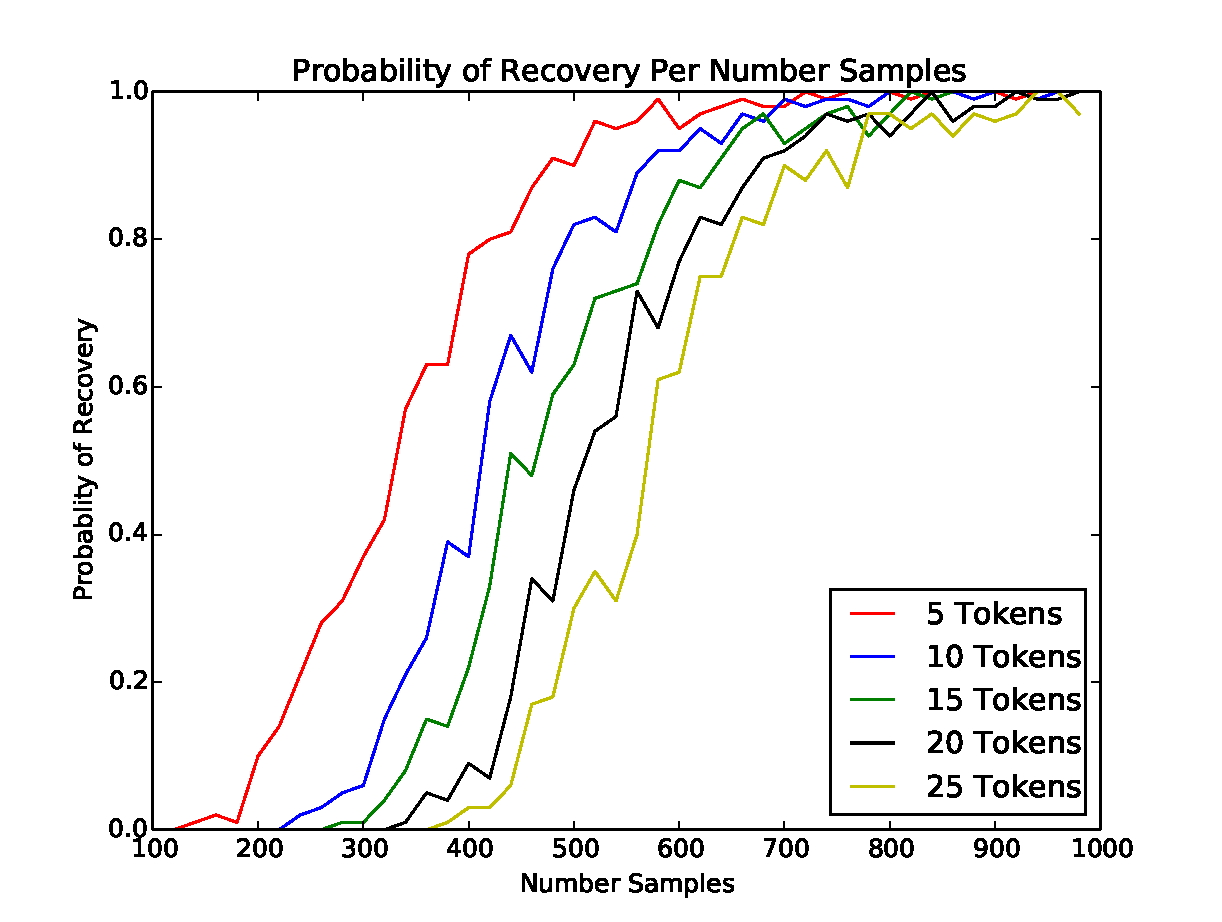
\includegraphics[width=3.5in]{./recovery_probability_per_samples.pdf}
	\caption{Recovery Probability}
	\label{fig:recovery_probability}
\end{figure}
For example, the red curve analyzes a sanitizer that blocks any string containing any one of five distinct patterns. This curve says that the sanitizer can be fully explained with almost 100\% accuracy with about 575 observations. Each observation requires running the sanitizer. This is much better than the alternative of running the sanitizer on strings that each contain a single pattern, which would require 4,970 observations (i.e. 4,970 invocations of the sanitizer). With only 300 observations, group testing will correctly identify the malicious patterns 50\% of the time. Since the curves increase rapidly, the additional number of observations to greatly increase the likelihood of success is quite small. This describes the power of group testing. By combining patterns in tests, we can greatly reduce the number of sanitizations required to fully explain the sanitizer with high likelihood of success.

We now discuss experiments on several of the sanitizers considered above in Section \ref{ss:sanitizers}. Of course, there is a large dependence on $p$ versus the number of samples. Recall that we need to observe enough blocked and unblocked strings in order to learn the sanitizer. We first consider whether Sanitizer 1 matches a single pattern ``$\sf{</alphanumerictext>}$". With $p=.01$, our framework outputs \textbf{Pattern 4902: $\sf{('</', '>')}$ has value 1.0}, i.e. it easily outputs the correct explanation of Sanitizer 1. NoteWith only 400 samples and a single malicious pattern, there were only two blocked strings to learn from.
A single malicious pattern is easy to catch, however, as long as $p$ is large enough to observe it in at least one string. 

We next consider Sanitizer 5, which matches the two patterns ``$\sf{</alphanumerictext>}$" and ``$\sf{(alphanumerictext)}$". Twelve out of the 400 sample strings were blocked, yet three patterns were found to explain the sanitizer; the framework output \textbf{Pattern 1136: $\sf{('(', ')')}$ has value 1.0, Pattern 3656: $\sf{('url(', ')')}$ has value 1.0, Pattern 4902: $\sf{('</', '>')}$ has value 1.0}. Even though we use delimiters, note that the pattern $\sf{('url(', ')')}$ contains as a sub-pattern $\sf{('(', ')')}$, so that both patterns are blocked for the same reasons. The framework currently does not differentiate between these patterns. This example shows successful explanation of the sanitizer with only 400 samples, along with one of the current drawbacks. When we similarly consider Sanitizer 7, we learn only two patterns with the framework outputting \textbf{Pattern 1136: $\sf{('(', ')')}$ has value 1.0, Pattern 4902: $\sf{('</', '>')}$}. Now, only nine strings were blocked. However, due to the delimiters included in the sanitizer, the correct explanation was found.
	
We finally consider Sanitizers 4 and 6 with the most malicious patterns. Running our framework on Sanitizer 4 (without delimiters) matches 376/400 random strings.  With so few unblocked strings, it is difficult for group testing to correctly explain the sanitizer, and indeed, the linear program results in a $\bx$ with 339 nonzero entries, rather than the four that correctly explain the sanitizer. Meanwhile, the same experiment with Sanitizer 6 (with delimiters) correctly explains the sanitizer with the output \textbf{Pattern 1: $\sf{script}$ has value 1.0, Pattern 12: $\sf{javascript:}$ has value 1.0, Pattern 1136: $\sf{('(', ')')}$ has value 1.0, Pattern 4902: $\sf{('</', '>')}$ has value 1.0}. 

This means that group testing can be a very powerful tool for explaining sanitizers. Furthermore, extending the tools we currently understand to account for ordering would make group testing even more powerful here.